\documentclass[11pt]{article}

\usepackage[T1]{fontenc}
\usepackage[utf8]{inputenc}
\usepackage[a4paper,margin=1in]{geometry}
\usepackage{amsmath,amssymb,amsthm,mathtools}
\usepackage{bm}
\usepackage{graphicx}
\usepackage{subcaption}
\usepackage{booktabs}
\usepackage{float}
\usepackage[colorlinks=true,linkcolor=blue,citecolor=blue,urlcolor=blue]{hyperref}

\graphicspath{{Partie_Mohamed/figures/}{Partie_Fatimetou/}{./}}

\newtheorem{theorem}{Th\'eor\`eme}[section]
\newtheorem{lemma}[theorem]{Lemme}
\newtheorem{proposition}[theorem]{Proposition}
\newtheorem{corollary}[theorem]{Corollaire}
\theoremstyle{remark}
\newtheorem{remark}[theorem]{Remarque}
\theoremstyle{definition}
\newtheorem{definition}[theorem]{D\'efinition}

\title{Localisation par filtrage de Kalman : du problème unidimensionnel à la navigation par odométrie}

\author{
  Fatimetou Narjah \and Mohamed Benloughmari
}
\date{}

\begin{document}

\maketitle

\section*{Introduction}

Le filtre de Kalman estime l'état d'un système dynamique en fusionnant un modèle d'évolution
avec des mesures bruitées. Ce rapport en étudie l'application à la localisation, en
progressant du cas unidimensionnel (position--vitesse) jusqu'à la navigation d'un robot par
odométrie. On y examine le comportement du filtre linéaire, puis du filtre étendu (EKF) face à
des mesures non linéaires, avant d'analyser l'effet des trous de mesure, des défaillances
capteur et du réglage des covariances $Q$ et $R$.

\section{Q0a --- Filtre de Kalman linéaire}

On note l'état $x = [p\ v]^\top$ (position, vitesse).

On construit le modèle d'évolution suivant

\begin{equation}
x_{k+1} = F\,x_k + w_k,
\qquad
F = \begin{bmatrix} 1 & \Delta T \\ 0 & 1 \end{bmatrix},
\qquad
w_k \sim \mathcal{N}\!\left(0,\ Q\right),
\quad
Q = \begin{bmatrix} 1 & 0 \\ 0 & 0.001 \end{bmatrix}
\end{equation}

avec $\Delta T = 1$.

On a le modèle d'observation suivant, où l'on mesure la position seule

\begin{equation}
y_k = H\,x_k + v_k,
\qquad
H = \begin{bmatrix} 1 & 0 \end{bmatrix},
\qquad
v_k \sim \mathcal{N}(0,\ R),\quad R = [1]
\end{equation}

Le problème est initialisé comme suit : réel $x_0 = [20,\ 12]^\top$, estimation
$\hat{x}_0 = [0,\ 10]^\top$, covariance $P_0 = \operatorname{diag}(100,\ 1)$.

\subsection{Récapitulatif des équations (rappel)}

\begin{equation}
\begin{aligned}
\text{Prédiction :}&& \hat{x}_{k|k-1} &= F\,\hat{x}_{k-1}, & P_{k|k-1} &= F P_{k-1} F^\top + Q \\[2pt]
\text{Innovation :}&& \nu_k &= y_k - H\,\hat{x}_{k|k-1}, & S_k &= H P_{k|k-1} H^\top + R \\[2pt]
\text{Gain :}&& K_k &= P_{k|k-1} H^\top S_k^{-1} \\[2pt]
\text{Correction :}&& \hat{x}_{k} &= \hat{x}_{k|k-1} + K_k\,\nu_k, & P_{k} &= (I - K_k H)\,P_{k|k-1}
\end{aligned}
\end{equation}

\begin{figure}[h]
    \centering
    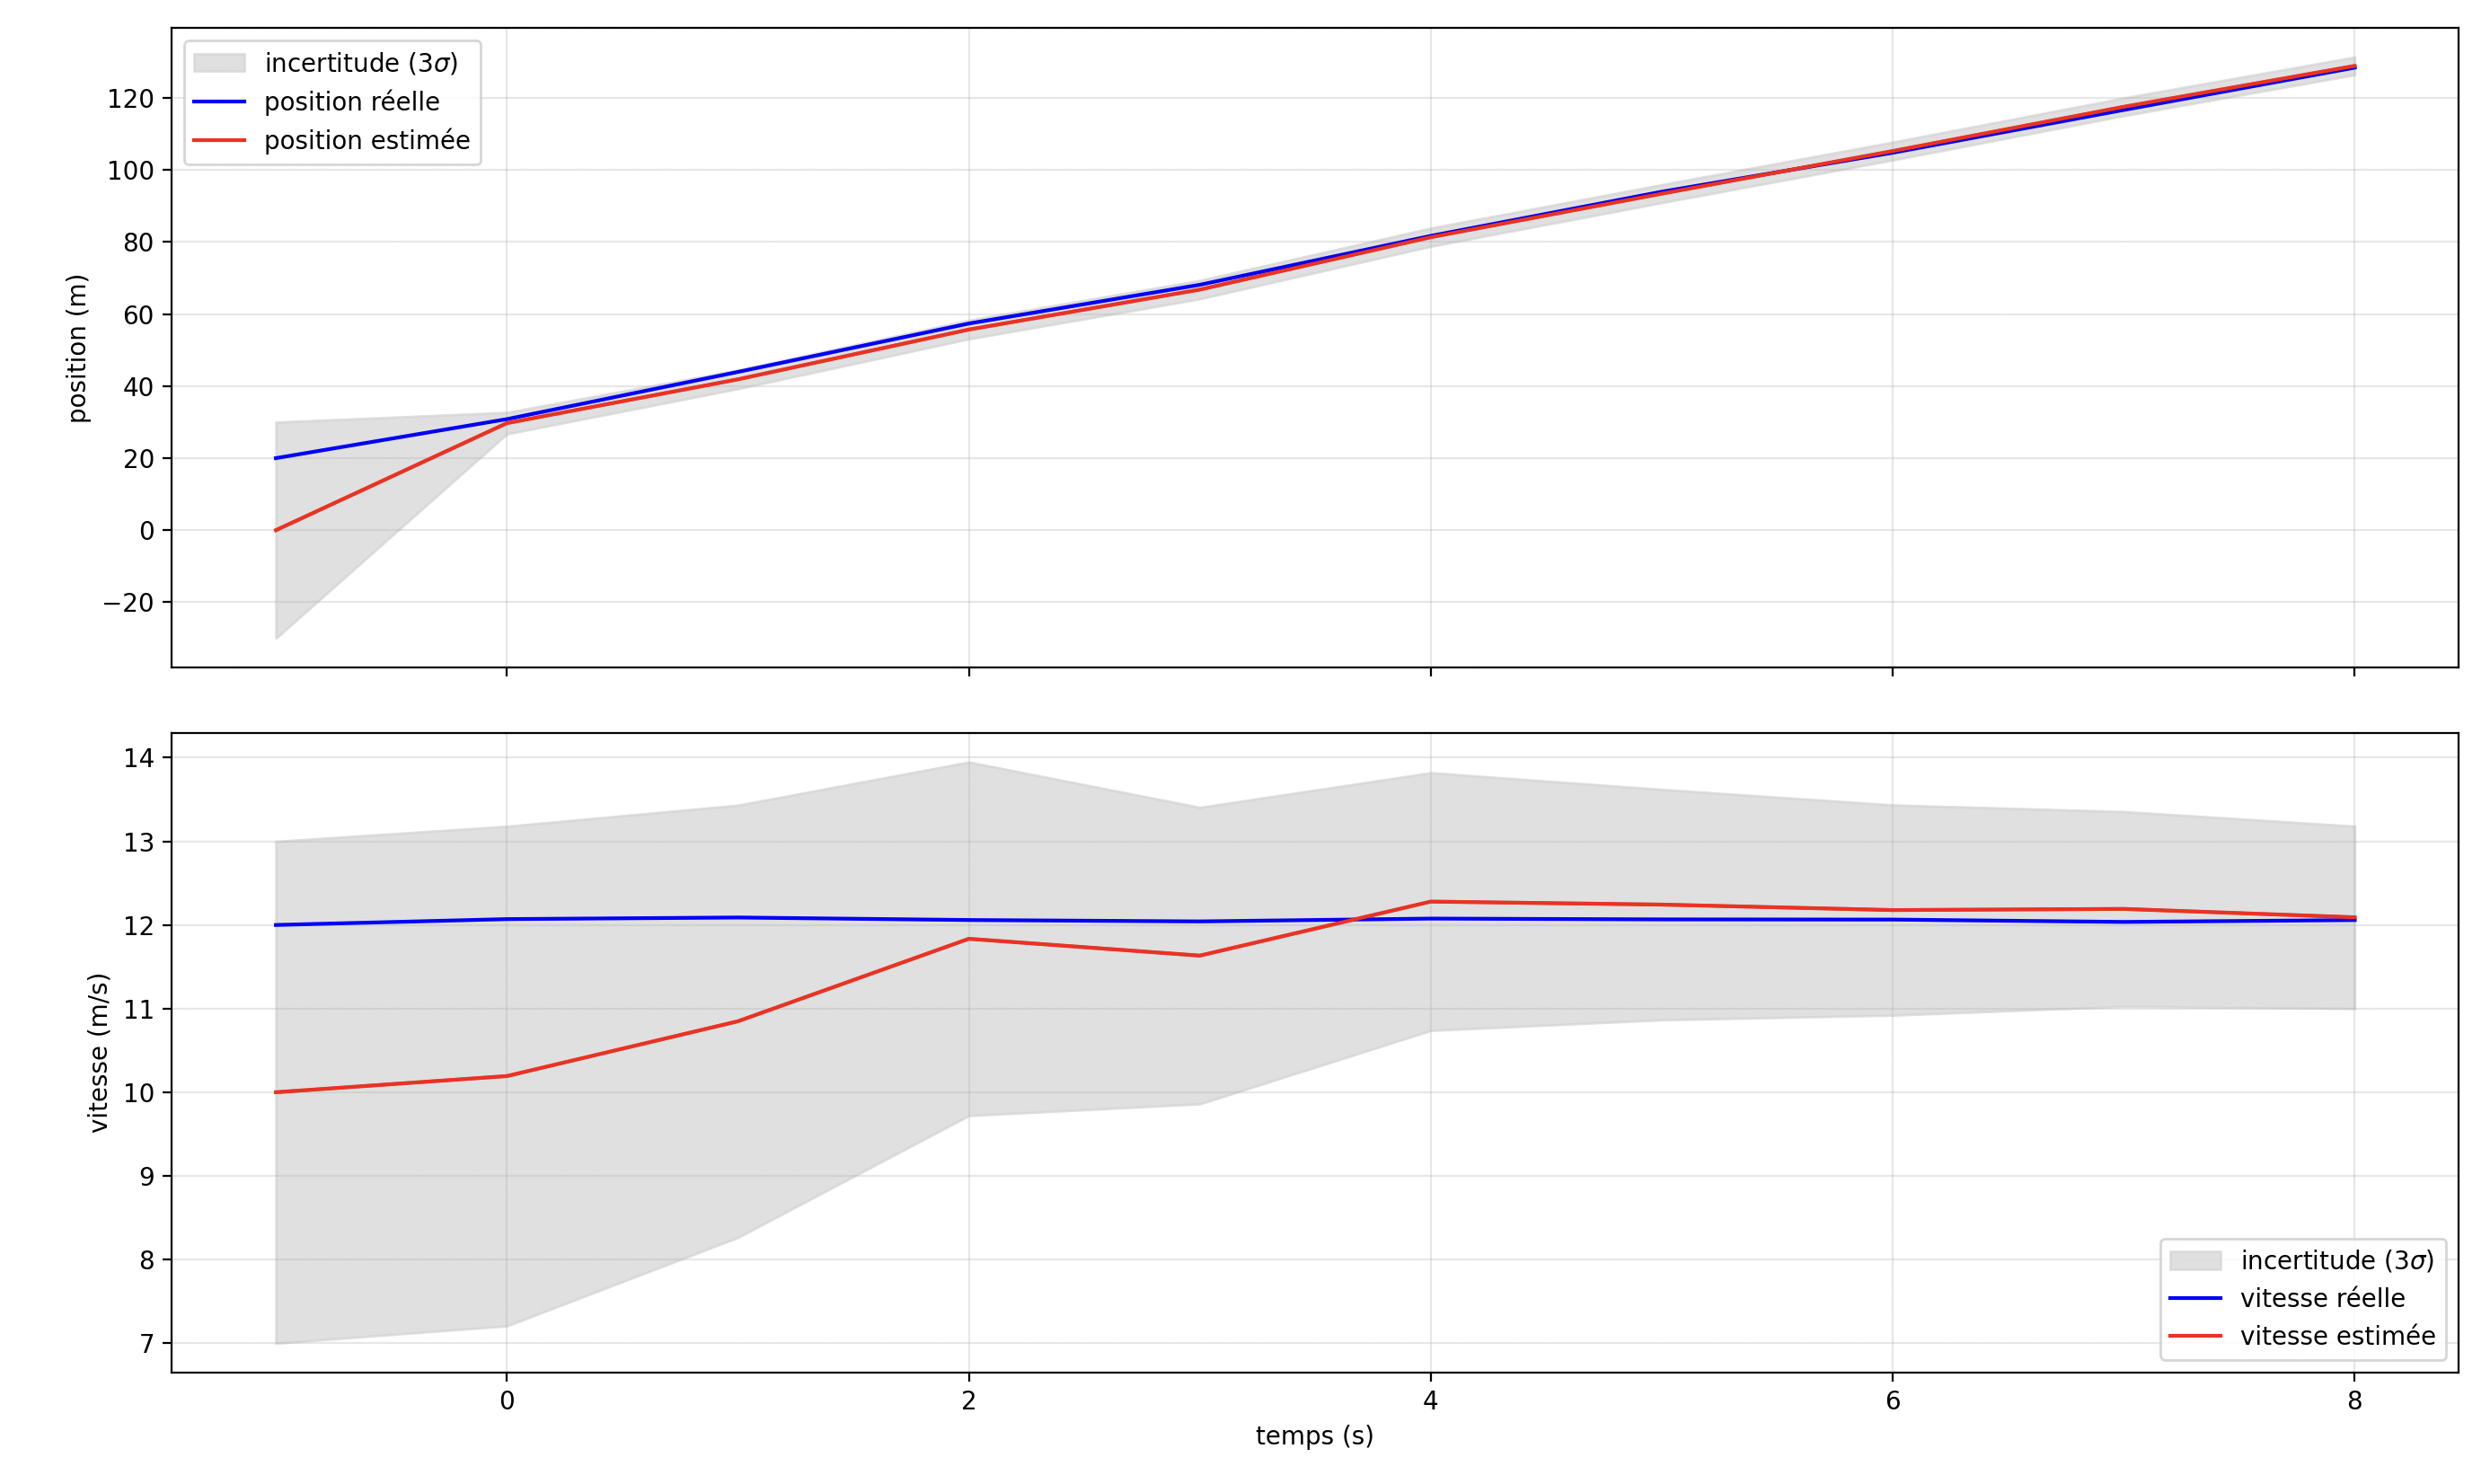
\includegraphics[width=0.8\textwidth]{question0a.png}
    \caption{Estimation de la position et de la vitesse (Q0a).}
    \label{fig:question0a}
\end{figure}

La figure \ref{fig:question0a} montre que l'estimation de la position converge rapidement vers
la position réelle, malgré un écart initial important. La vitesse n'étant pas directement
observée, elle est estimée indirectement à partir de l'évolution temporelle des mesures de
position. L'incertitude sur la vitesse reste ainsi plus importante que celle sur la position,
notamment au début, avant de diminuer progressivement. Le filtre parvient néanmoins à
reconstruire correctement la vitesse et à faire converger l'ensemble de l'état vers la
trajectoire réelle.

\section{Q0b --- Filtre de Kalman étendu}

Après avoir étudié le cas linéaire, on quitte désormais ce cadre : on considère un objet qui
se déplace sur l'axe $x$, d'état $x = [s\ v]^\top$ (position, vitesse), mais dont la mesure
n'est plus linéaire. En effet, un capteur placé en $(x_s, y_s) = (0, -20)$ mesure un
angle bruité vers l'objet, et non plus la position, sans aucune mesure de distance.
C'est pourquoi on a recours au filtre de Kalman étendu (EKF), qui linéarise localement le
modèle d'observation.

Modèle d'évolution. Tout d'abord, l'évolution reste linéaire ($\Delta T = 1$) :

\begin{equation}
x_{k+1} = F x_k + w_k,
\qquad
F = \begin{bmatrix} 1 & \Delta T \\ 0 & 1 \end{bmatrix},
\qquad
w_k \sim \mathcal{N}(0, Q),
\quad
Q = \begin{bmatrix} 0.0001 & 0 \\ 0 & 0.01 \end{bmatrix}
\end{equation}

Modèle d'observation. Ensuite, l'observation devient non linéaire :

\begin{equation}
z_k = h(s_k) + v_k,
\qquad
h(s) = \operatorname{atan2}\!\big(-y_s,\ s - x_s\big) = \operatorname{atan2}(20,\ s),
\qquad
v_k \sim \mathcal{N}(0, R),
\end{equation}

avec $R = (1^\circ\ \text{en radians})^2 \approx (0.01745)^2 \approx 3.05\times 10^{-4}$.

Jacobienne d'observation. L'EKF linéarise $h$ autour de l'état courant :

\begin{equation}
H = \frac{\partial h}{\partial x} =
\begin{bmatrix} \dfrac{\partial h}{\partial s} & \dfrac{\partial h}{\partial v} \end{bmatrix}
=
\begin{bmatrix} h_s & 0 \end{bmatrix},
\qquad
h_s = \frac{y_s}{(s - x_s)^2 + y_s^2} = \frac{-20}{s^2 + 400}
\end{equation}

Un point essentiel apparaît ici : $h_s$ dépend de $s$ et tend vers $0$ quand l'objet
s'éloigne du capteur ($s \to \infty$). Autrement dit, la mesure devient de moins en moins
informative sur la position.

Initialisation. Enfin, le problème est initialisé avec le réel $x_0 = [2,\ 4]^\top$,
l'estimation $\hat{x}_0 = [0,\ 5]^\top$ et $P_0 = \operatorname{diag}(100,\ 1)$.

\subsection{Récapitulatif de l'EKF}

\begin{equation}
\begin{aligned}
\text{Prédiction :}&& \hat{x}_{k|k-1} &= f(\hat{x}_{k-1|k-1}), & P_{k|k-1} &= F P_{k-1|k-1} F^\top + Q \\[2pt]
\text{Innovation :}&& \nu_k &= z_k - h(\hat{x}_{k|k-1}), & S_k &= H P_{k|k-1} H^\top + R \\[2pt]
\text{Gain :}&& K_k &= P_{k|k-1} H^\top S_k^{-1} \\[2pt]
\text{Correction :}&& \hat{x}_{k|k} &= \hat{x}_{k|k-1} + K_k \nu_k, & P_{k|k} &= (I - K_k H) P_{k|k-1}
\end{aligned}
\end{equation}

\begin{figure}[h]
    \centering
    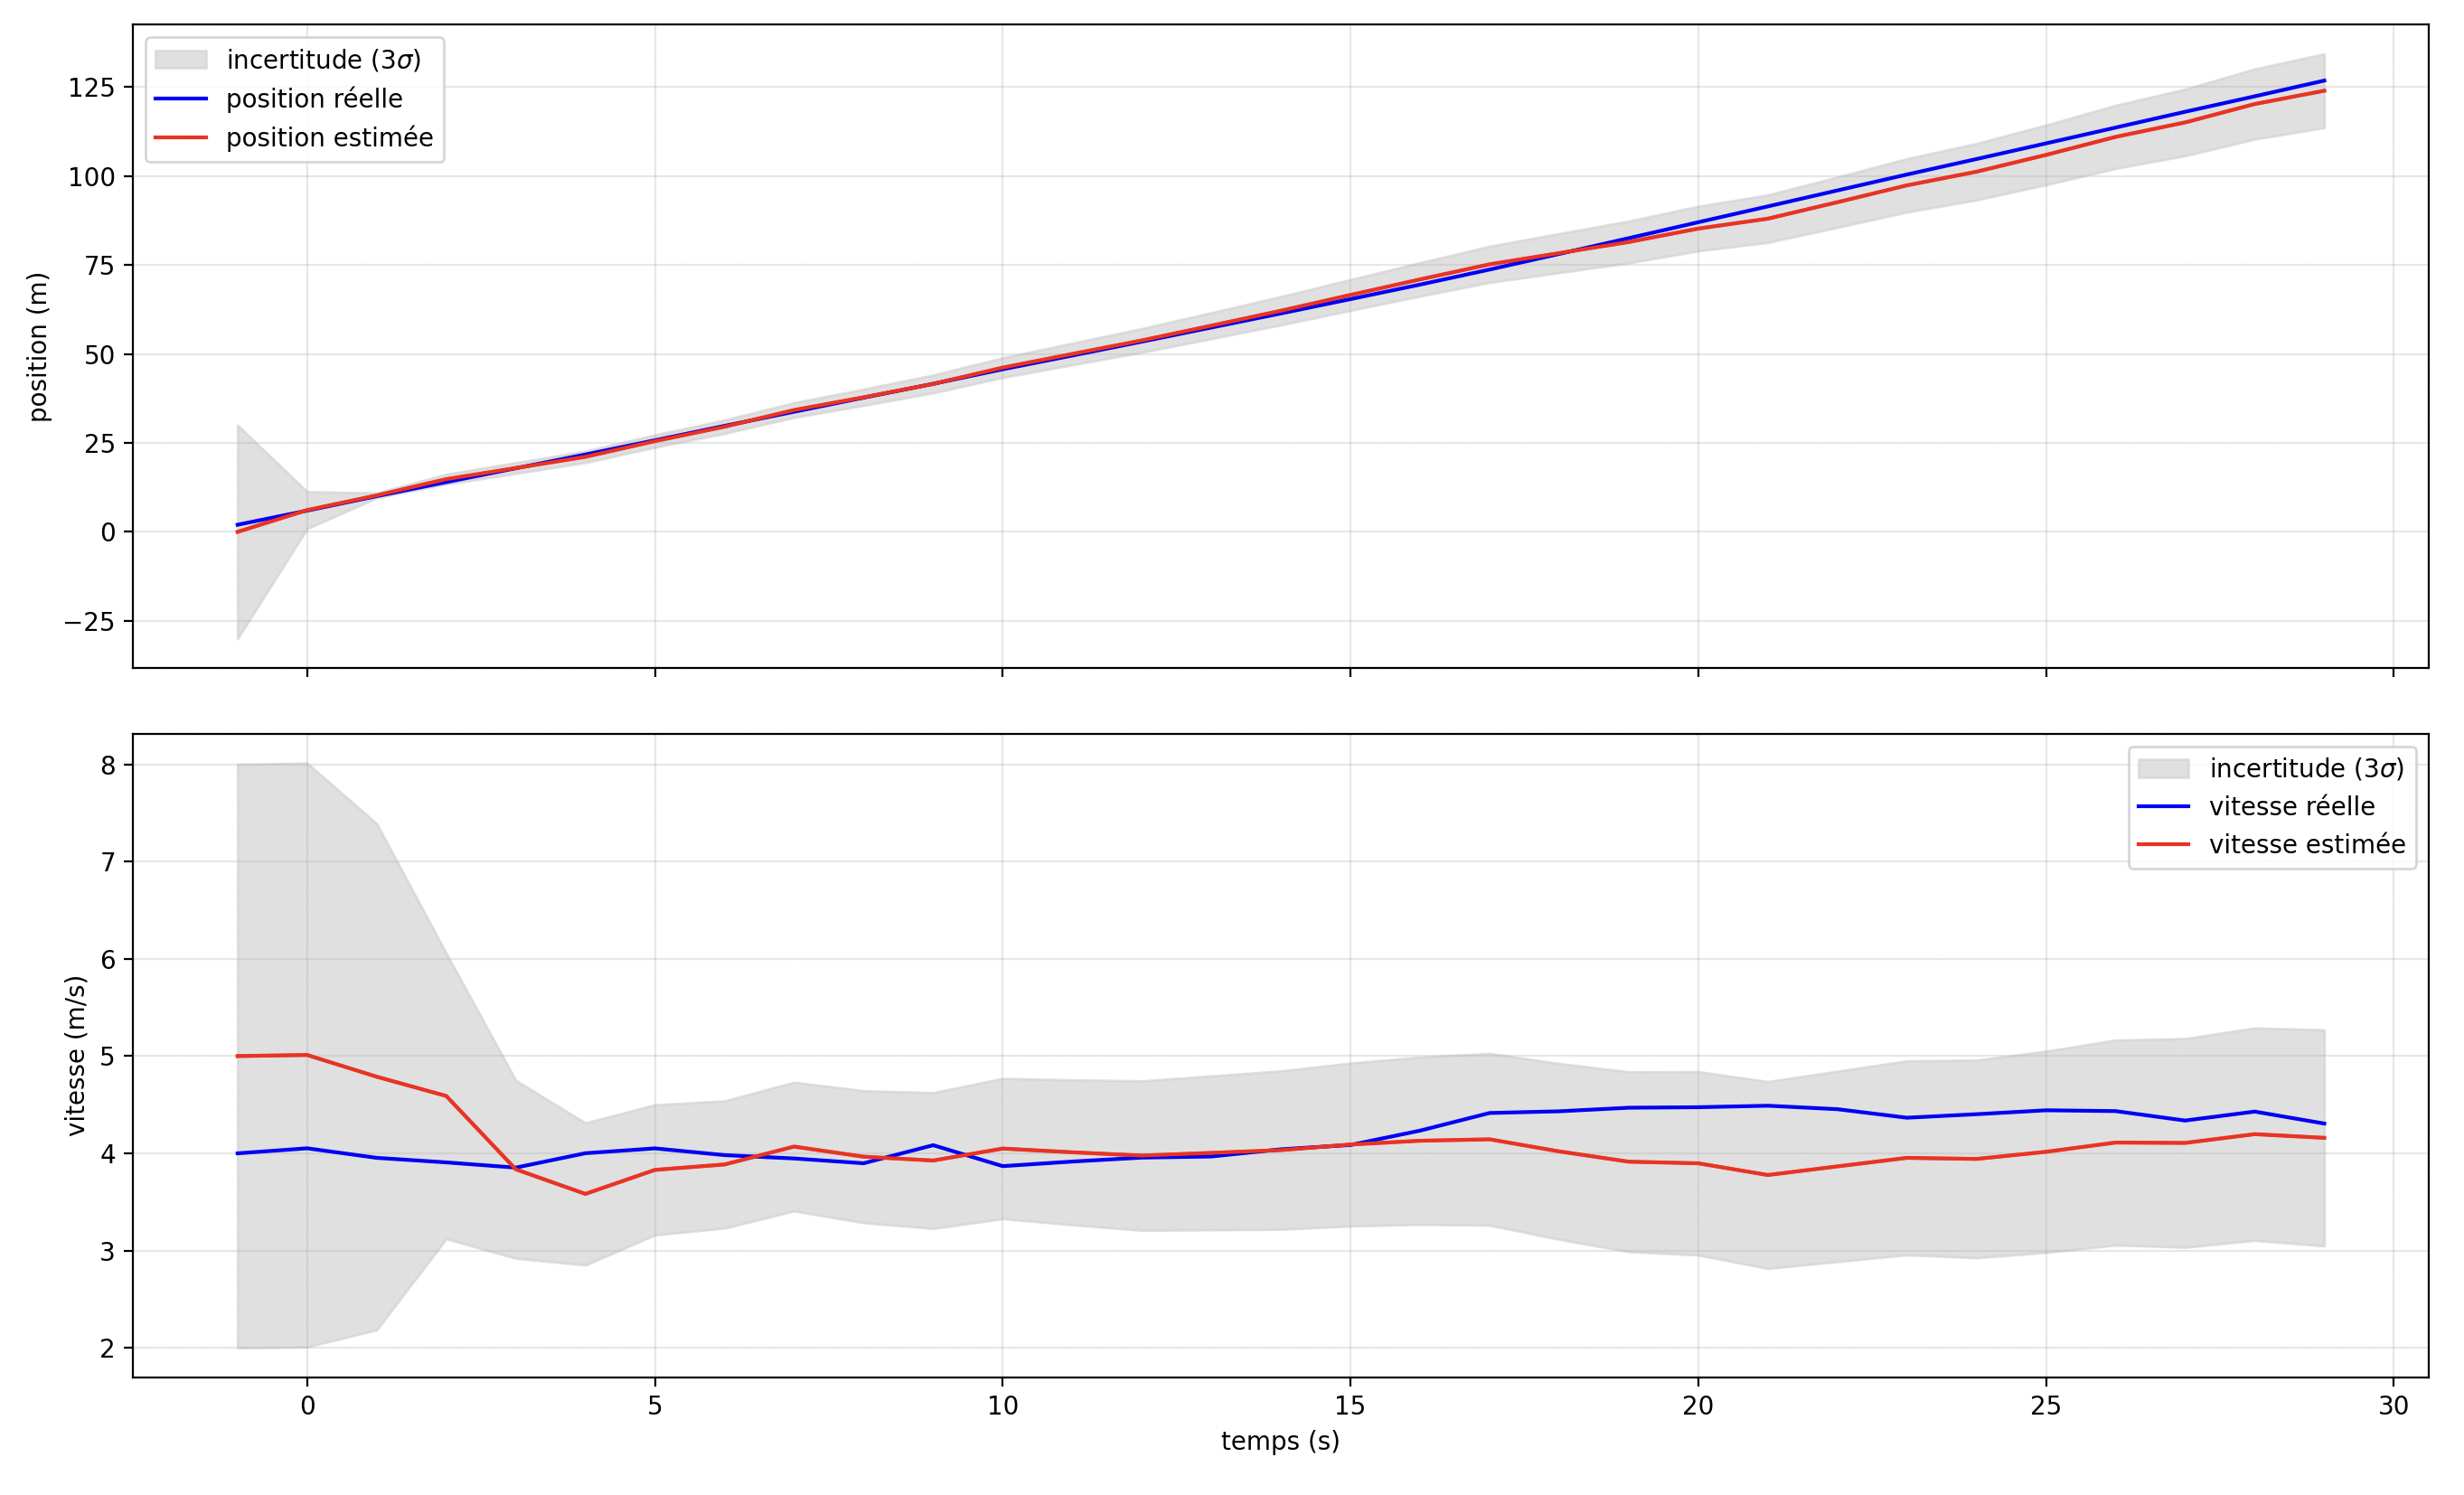
\includegraphics[width=0.8\textwidth]{question0b.png}
    \caption{Estimation de la position et de la vitesse avec une mesure d'angle uniquement (Q0b).}
    \label{fig:question0b}
\end{figure}

La figure \ref{fig:question0b} révèle un comportement opposé au cas précédent : l'incertitude,
qu'il s'agisse de la position ou de la vitesse, croît avec le temps au lieu de
converger. Ainsi, après une phase initiale de convergence, l'estimation diverge peu à
peu.

\subsection{Explication}

Pour comprendre cette divergence, on note la covariance $P_k =
\begin{bmatrix} a_k & b_k \\ b_k & c_k \end{bmatrix}$, avec $a_k = \operatorname{var}(s_k)$,
$c_k = \operatorname{var}(v_k)$ (variance de vitesse) et $b_k = \operatorname{cov}(s_k, v_k)$.

Prédiction ($P_{k|k-1} = F P_{k-1} F^\top + Q$, avec $q_p = 10^{-4}$, $q_v = 10^{-2}$) :

\begin{equation}
a_{k|k-1} = a_{k-1} + 2b_{k-1} + c_{k-1} + q_p,
\qquad
b_{k|k-1} = b_{k-1} + c_{k-1},
\qquad
c_{k|k-1} = c_{k-1} + q_v .
\end{equation}

Correction avec $H = [h_s\ 0]$ :

\begin{equation}
S_k = h_s^2\, a_{k|k-1} + R,
\qquad
K_k = P_{k|k-1} H^\top S_k^{-1}
= \frac{1}{S_k}\begin{bmatrix} h_s\,a_{k|k-1} \\ h_s\,b_{k|k-1} \end{bmatrix}.
\end{equation}

Le bloc $(2,2)$ de $P_k = (I - K_k H) P_{k|k-1}$ donne alors la nouvelle variance de vitesse :

\begin{equation}
c_k = c_{k|k-1} - \frac{h_s^2\, b_{k|k-1}^2}{S_k}
= c_{k|k-1} - \frac{h_s^2\, b_{k|k-1}^2}{h_s^2\, a_{k|k-1} + R}.
\end{equation}

D'où la récurrence complète :

\begin{equation}
\boxed{\,c_k = c_{k-1} + q_v - \frac{h_s^2\,(b_{k-1} + c_{k-1})^2}{\,h_s^2\,(a_{k-1} + 2b_{k-1} + c_{k-1} + q_p) + R\,}\,}
\end{equation}

Lecture de la formule

\begin{itemize}
\item Terme $+q_v$ : à chaque prédiction, le bruit de dynamique injecte $q_v = 10^{-2}$
   d'incertitude sur la vitesse. C'est le moteur de la croissance.

\item Terme de correction $-\dfrac{h_s^2 b_{k|k-1}^2}{S_k}$ : c'est la seule chose qui
   « tire » la variance de vitesse vers le bas. Or la mesure d'angle n'observe pas
   directement la vitesse ($H$ a une composante nulle sur $v$) : la vitesse n'est corrigée
   qu'indirectement, via sa covariance croisée $b$ avec la position.

\item Rôle de $h_s \to 0$ : quand l'objet s'éloigne, $h_s = -20/(s^2+400) \to 0$. Alors
   le numérateur $h_s^2 b_{k|k-1}^2 \to 0$ (et $S_k \to R$, non nul), donc le terme de
   correction s'annule. La récurrence se réduit à

   \begin{equation}
   c_k \approx c_{k|k-1} = c_{k-1} + q_v .
   \end{equation}

   La variance de vitesse croît alors linéairement, avec une pente $q_v = 10^{-2}$.
\end{itemize}

\section{Q1.1 --- Localisation GNSS : modèle et trou de mesure}

Après avoir traité les problèmes unidimensionnels, on généralise désormais le filtre à un
objet qui se déplace dans $\mathbb{R}^3$. Concrètement, on applique la classe
\texttt{KalmanFilter} à une localisation GNSS (de type GPS) simplifiée : seules les
trois coordonnées de position sont mesurées, et l'on suppose ces mesures
indépendantes en choisissant un pas de temps $\Delta T$ suffisamment grand.

\subsection{Modèle}

État. L'état regroupe la position et la vitesse :

\begin{equation}
x_k = \begin{bmatrix} p_x & p_y & p_z & v_x & v_y & v_z \end{bmatrix}^\top \in \mathbb{R}^6 .
\end{equation}

Modèle d'évolution. En l'absence de commande, la dynamique est à vitesse
quasi-constante :

\begin{equation}
x_{k+1} = F\, x_k + w_k,
\qquad
w_k \sim \mathcal{N}(0, Q),
\end{equation}

avec la matrice de transition ($\Delta T = 1$) :

\begin{equation}
F =
\begin{bmatrix}
1 & 0 & 0 & \Delta T & 0 & 0 \\
0 & 1 & 0 & 0 & \Delta T & 0 \\
0 & 0 & 1 & 0 & 0 & \Delta T \\
0 & 0 & 0 & 1 & 0 & 0 \\
0 & 0 & 0 & 0 & 1 & 0 \\
0 & 0 & 0 & 0 & 0 & 1
\end{bmatrix}
=
\begin{bmatrix}
I_3 & \Delta T\,I_3 \\[2pt]
0 & I_3
\end{bmatrix},
\end{equation}

et la covariance du bruit de dynamique :

\begin{equation}
Q = \operatorname{diag}(10^{-4},\ 10^{-4},\ 10^{-4},\ 10^{-2},\ 10^{-2},\ 10^{-2}).
\end{equation}

Précisons le sens de ce choix : le bruit sur la vitesse ($10^{-2}$) est nettement plus grand
que celui sur la position ($10^{-4}$). En d'autres termes, le modèle « laisse de la latitude »
à la vitesse, ce qui lui permet de suivre un objet dont la vitesse réelle n'est pas
rigoureusement constante.

Modèle d'observation. On observe les trois coordonnées de position :

\begin{equation}
y_k = H\, x_k + v_k,
\qquad
v_k \sim \mathcal{N}(0, R),
\end{equation}

\begin{equation}
H =
\begin{bmatrix}
1 & 0 & 0 & 0 & 0 & 0 \\
0 & 1 & 0 & 0 & 0 & 0 \\
0 & 0 & 1 & 0 & 0 & 0
\end{bmatrix}
=
\begin{bmatrix}
I_3 & 0_{3\times 3}
\end{bmatrix},
\qquad
R = 100\,I_3
\quad (\sigma_{\text{mesure}} = 10\ \text{m}).
\end{equation}

Initialisation. Enfin, l'état vrai initial vaut
$x_0^{\text{true}} = [20,\,-10,\,5,\,0,\,5,\,0]^\top$. De son côté, le filtre démarre de
l'estimation $x_0 = 0_6$, avec la forte incertitude initiale suivante :

\begin{equation}
P_0 = \operatorname{diag}(10^4,\ 10^4,\ 10^4,\ 10^2,\ 10^2,\ 10).
\end{equation}

\subsection{Trou de mesure}

On introduit à présent un trou de mesure : la mesure est supprimée entre $t = 10$ et
$t = 20$ (exclus), au moyen du masque \texttt{has\_measure[11:21] = False}. Pendant cette
fenêtre, la boucle saute les étapes de simulation et de correction, de sorte que seules les
prédictions sont exécutées, si bien que

\begin{equation}
\hat{x}_{k+1} = \hat{x}_{k+1|k} = F\,\hat{x}_{k},
\qquad
P_{k+1} = P_{k+1|k} = F\,P_{k}\,F^\top + Q .
\end{equation}

\begin{figure}[h]
    \centering
    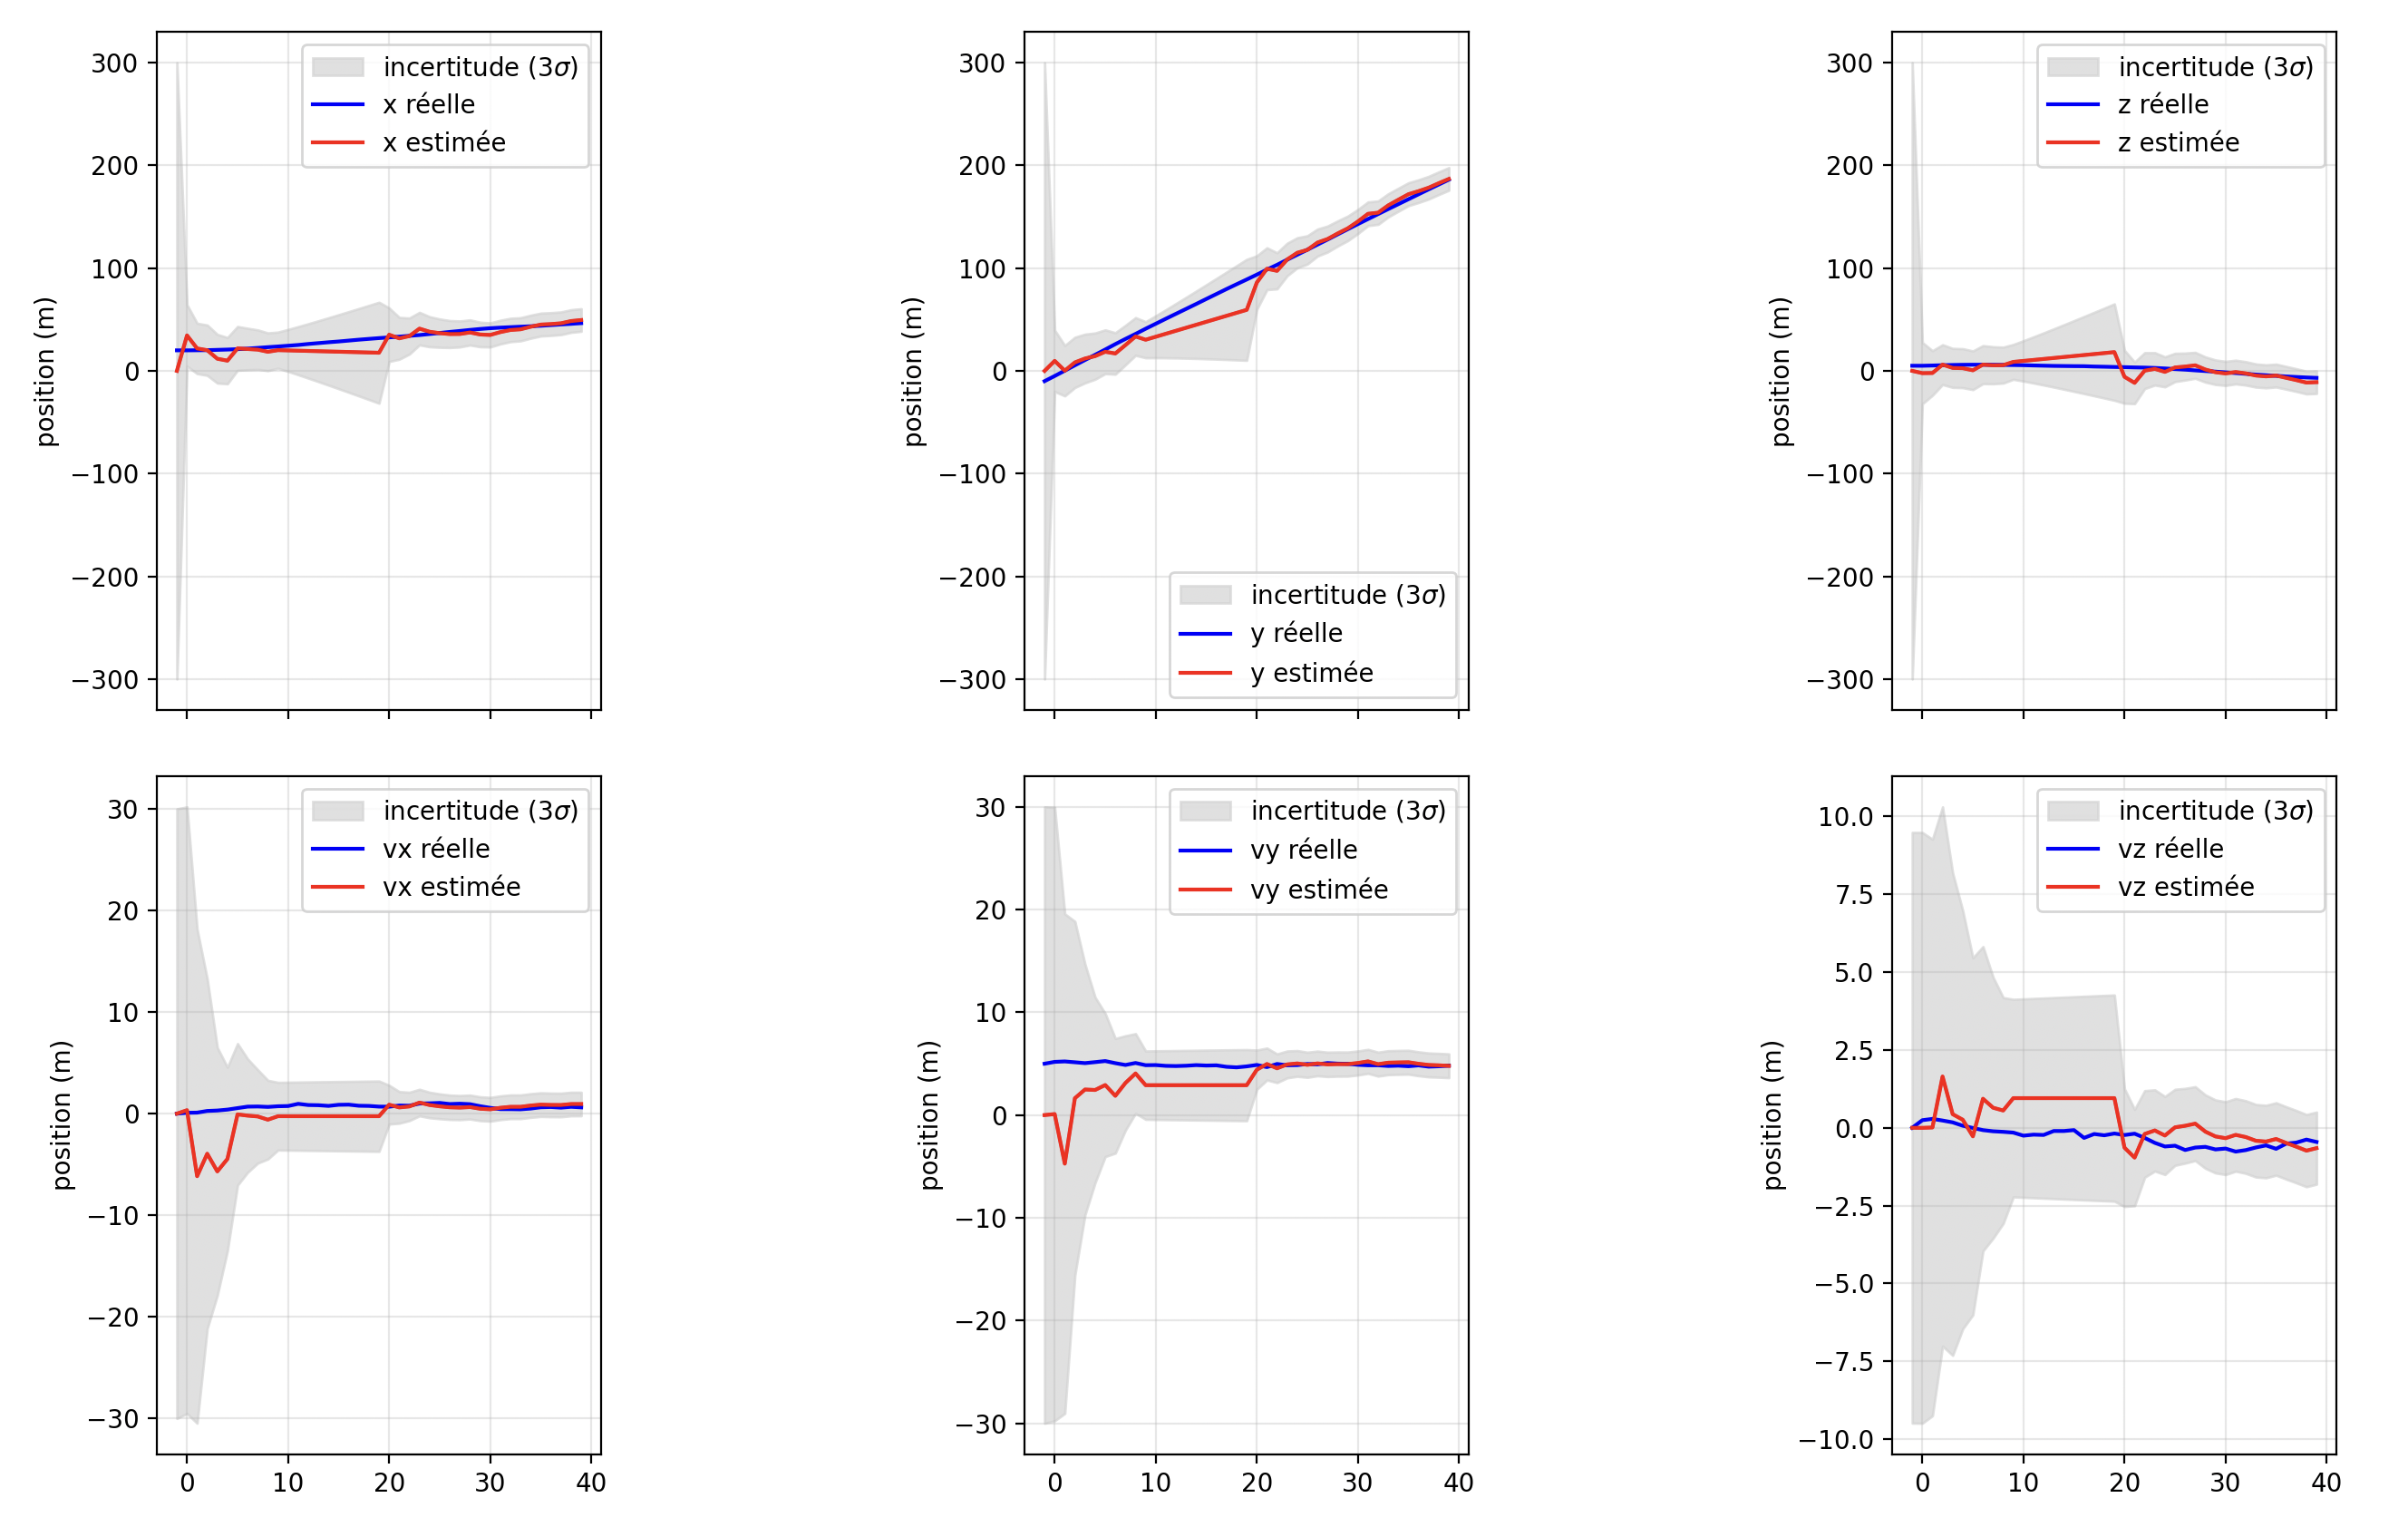
\includegraphics[width=0.8\textwidth]{trou_de_mesureq1.png}
    \caption{Localisation GNSS avec un trou de mesure entre $t=10$ et $t=20$.}
    \label{fig:trou_mesure}
\end{figure}

La figure \ref{fig:trou_mesure} montre que, pendant le trou, l'incertitude sur la
position augmente nettement, tandis que celle sur la vitesse reste quasi
constante. Autrement dit, privé de mesure, le filtre se contente d'extrapoler à partir de son
modèle de mouvement : la covariance $P$ n'étant plus recadrée, elle ne peut que croître.

\subsection{Explication}

On observe ainsi, sur les bandes $\pm 3\sigma$, que la variance de position croît tandis que
la variance de vitesse reste quasi constante. On le justifie à présent par un calcul exact,
mené avec la matrice $F$ complète ($6\times 6$).

Écriture par blocs. On note l'état $x = [p\ v]^\top$, où $p = [p_x\ p_y\ p_z]^\top$
désigne la position et $v = [v_x\ v_y\ v_z]^\top$ la vitesse. Avec $\Delta T = 1$ :

\begin{equation}
F =
\begin{bmatrix}
I_3 & I_3 \\[2pt]
0_3 & I_3
\end{bmatrix},
\qquad
Q =
\begin{bmatrix}
q_p I_3 & 0_3 \\[2pt]
0_3 & q_v I_3
\end{bmatrix},
\quad q_p = 10^{-4},\ q_v = 10^{-2}.
\end{equation}

De la même manière, on partitionne la covariance complète :

\begin{equation}
P_k =
\begin{bmatrix}
P_{pp,k} & P_{pv,k} \\[2pt]
P_{vp,k} & P_{vv,k}
\end{bmatrix},
\end{equation}

où $P_{pp,k}$ est la variance de position ($3\times 3$), $P_{vv,k}$ celle de vitesse, et
$P_{pv,k} = P_{vp,k}^\top$ la covariance croisée position--vitesse.

Pendant le trou, on a une prédiction seule : $P_{k+1} = F P_k F^\top + Q$. Le produit
$F P_k F^\top$ donne :

\begin{equation}
F P_k F^\top =
\begin{bmatrix}
P_{pp,k} + P_{pv,k} + P_{vp,k} + P_{vv,k} & P_{pv,k} + P_{vv,k} \\[2pt]
P_{vp,k} + P_{vv,k} & P_{vv,k}
\end{bmatrix},
\end{equation}

d'où les récurrences par blocs :

\begin{equation}
\boxed{\begin{aligned}
P_{pp,k+1} &= P_{pp,k} + P_{pv,k} + P_{vp,k} + P_{vv,k} + q_p\,I_3 \\[2pt]
P_{pv,k+1} &= P_{pv,k} + P_{vv,k} \\[2pt]
P_{vp,k+1} &= P_{vp,k} + P_{vv,k} \\[2pt]
P_{vv,k+1} &= P_{vv,k} + q_v\,I_3 .
\end{aligned}}
\end{equation}

Découplage par axe. Puisque $F$, $Q$, $H$ et $R$ sont diagonales par blocs (un bloc
$2\times 2$ par axe), tous les blocs $P_{pp}$, $P_{pv}$, $P_{vp}$, $P_{vv}$ sont eux-mêmes
diagonaux. Chaque axe $(x,y,z)$ suit donc une récurrence scalaire indépendante ;
ainsi, pour un axe donné, en posant

\begin{equation}
a_k = (P_{pp,k})_{ii},\qquad b_k = (P_{pv,k})_{ii} = (P_{vp,k})_{ii},\qquad c_k = (P_{vv,k})_{ii},
\end{equation}

les récurrences par blocs se réduisent exactement à :

\begin{equation}
\boxed{\begin{aligned}
a_{k+1} &= a_k + 2b_k + c_k + q_p \\[2pt]
b_{k+1} &= b_k + c_k \\[2pt]
c_{k+1} &= c_k + q_v .
\end{aligned}}
\end{equation}

Variance de vitesse : croissance linéaire, pente faible. La troisième récurrence
donne immédiatement

\begin{equation}
c_k = c_0 + k\,q_v .
\end{equation}

La variance de vitesse croît donc linéairement en $k$, avec une pente $q_v = 10^{-2}$
très faible. Sur 10 pas, $c_{10} - c_0 = 0.1$, à comparer à $c_0 \approx 0.14$ (régime
stationnaire) : l'écart-type $\sigma_v(k) = \sqrt{c_0 + k\,q_v}$ varie peu, ce qui explique que
la bande $\pm 3\sigma_v$ semble constante.

Variance de position : croissance quadratique. De $b_{k+1} = b_k + c_k$, on déduit

\begin{equation}
b_k = b_0 + k\,c_0 + q_v\,\frac{k(k-1)}{2} .
\end{equation}

En injectant dans la récurrence de $a$ puis en sommant, on obtient la forme fermée :

\begin{equation}
\boxed{\,a_k = a_0 + (2b_0 + c_0 + q_p)\,k + c_0\,k(k-1) + q_v\,\frac{k(k-1)(2k-1)}{6}\,}
\end{equation}

Le terme dominant est quadratique : $a_k \sim c_0\,k^2$ (le terme cubique en $q_v$ est
négligeable devant lui). En effet, la dérivée seconde discrète

\begin{equation}
\Delta^2 a_k = \Delta a_{k+1} - \Delta a_k = 2c_k + q_v = 2c_0 + q_v + 2 q_v k \approx 2c_0
\end{equation}

est constante au premier ordre : c'est la signature d'une croissance quadratique. L'écart-type,
lui, croît linéairement : $\sigma_p(k) = \sqrt{a_k} \sim \sqrt{c_0}\ k$.

Conclusion. C'est donc bien l'écart-type $\sigma$ (la grandeur tracée) qui est
linéaire pour la position et quasi constant pour la vitesse. En termes de variance, la
position est quadratique en $k$ (terme dominant $c_0 k^2$), tandis que la vitesse est
linéaire, mais avec une pente $q_v$ si faible qu'elle paraît constante.

\subsection{Interprétation}

Ce comportement a une lecture physique directe. D'une part, la vitesse se propage par simple
ajout de bruit ($+q_v$ à chaque pas) : sa variance augmente donc d'une constante à
chaque pas, de façon régulière. D'autre part, la position intègre la vitesse
($p_{k+1} = p_k + v_k$) : son incertitude s'accumule, car chaque pas ajoute
l'incertitude de vitesse déjà accumulée, d'où la croissance accélérée (quadratique) de sa
variance.

Il s'agit là du comportement typique de la navigation à l'estime (dead reckoning)
sans recalage externe : privé de mesure, le filtre « navigue à l'aveugle », et ses erreurs ne
font que s'additionner d'un pas à l'autre sans jamais être remises à zéro. Dès la reprise des
mesures, l'innovation est grande et la covariance élevée : le gain $K$ redevient alors
important, le filtre recale brutalement l'estimation, puis $P$ redescend vers son
régime stationnaire.

\section{Q1.2 --- Influence du bruit de dynamique Q}

Dans cette expérience, nous étudions l'influence de la matrice $Q$,
qui représente le bruit associé au modèle dynamique. La covariance
prédite est donnée par :

\begin{equation}
P_{k|k-1}=F P_{k-1|k-1}F^T+Q.
\end{equation}

Initialement,

\begin{equation}
Q_{\mathrm{initial}}
=
\operatorname{diag}
(10^{-4},10^{-4},10^{-4},10^{-2},10^{-2},10^{-2}).
\end{equation}

Nous avons ensuite augmenté $Q$ d'un facteur $100$ :

\begin{equation}
Q_{\mathrm{nouveau}}=100Q_{\mathrm{initial}}
=
\operatorname{diag}(10^{-2},10^{-2},10^{-2},1,1,1).
\end{equation}

\begin{figure}[H]
    \centering
    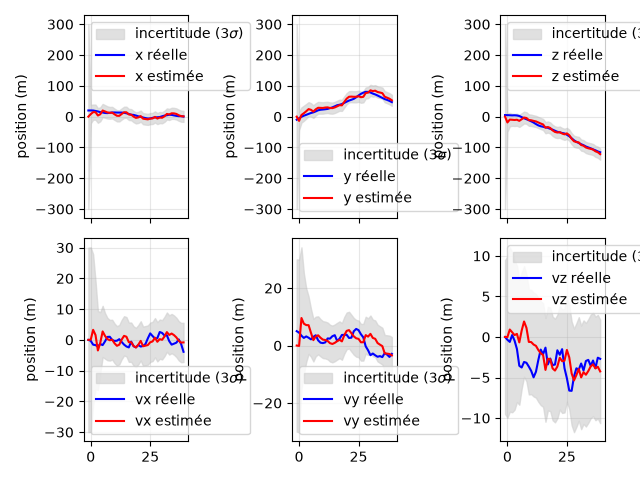
\includegraphics[width=0.95\textwidth]{Q1_variation_Q.png}
    \caption{Influence de l'augmentation du bruit de dynamique $Q$.}
    \label{fig:q1_Q}
\end{figure}

On observe que l'augmentation de $Q$ élargit les bandes d'incertitude,
car la covariance prédite augmente :

\[
Q\uparrow
\quad\Longrightarrow\quad
P_{k|k-1}\uparrow
\quad\Longrightarrow\quad
\sigma\uparrow.
\]

L'effet est particulièrement visible sur les vitesses $v_x$, $v_y$ et
$v_z$. En effet, les mesures GNSS observent directement la position
mais pas la vitesse :

\begin{equation}
H=
\begin{bmatrix}
I_3 & 0_3
\end{bmatrix}.
\end{equation}

Les positions sont donc régulièrement corrigées par les mesures, tandis
que les vitesses sont estimées indirectement à partir du modèle dynamique.
Elles sont ainsi plus sensibles à l'augmentation du bruit de processus
$Q$. L'information de position permet néanmoins de corriger indirectement
les vitesses grâce au couplage entre position et vitesse dans la matrice
$F$.

\section{Q1.3 --- Influence du bruit de mesure R}

Dans cette expérience, on fait varier la matrice $R$, qui représente
le bruit associé aux mesures GNSS.

La covariance de l'innovation est donnée par :

\begin{equation}
S_k = HP_{k|k-1}H^T+R.
\end{equation}

Le gain de Kalman est :

\begin{equation}
K_k =
P_{k|k-1}H^T
\left(HP_{k|k-1}H^T+R\right)^{-1}.
\end{equation}

Lorsque $R$ augmente, $S_k$ augmente et le gain de Kalman $K_k$ diminue.
Le filtre accorde donc moins de confiance aux mesures GNSS et davantage
à la prédiction issue du modèle dynamique.

\begin{figure}[H]
    \centering
    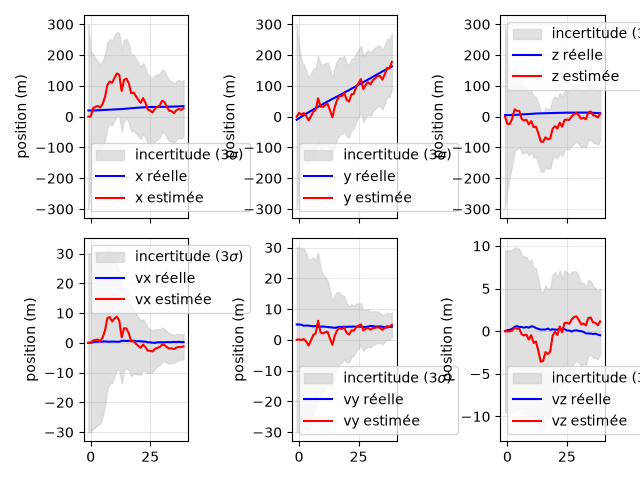
\includegraphics[width=0.95\textwidth]{Q1_variation_R.png}
    \caption{Influence de la variation du bruit de mesure $R$ sur
    l'estimation et l'incertitude du filtre.}
    \label{fig:q1_R}
\end{figure}

On observe que l'augmentation de $R$ entraîne une augmentation des bandes
d'incertitude, à la fois pour les positions et pour les vitesses. En effet,
la covariance après correction est moins réduite lorsque le gain de Kalman
diminue :

\begin{equation}
P_{k|k}=(I-K_kH)P_{k|k-1}.
\end{equation}

Les positions sont directement mesurées par le GNSS, mais lorsque $R$ est
grand, ces mesures sont considérées comme peu fiables et corrigent moins
efficacement la prédiction. La position reste donc plus incertaine.

Les vitesses ne sont pas mesurées directement. Elles dépendent de
l'information de position pour être corrigées indirectement. Lorsque les
mesures de position deviennent moins fiables à cause de l'augmentation de
$R$, cette correction indirecte des vitesses devient également moins
efficace. L'incertitude augmente donc aussi pour $v_x$, $v_y$ et $v_z$.

Ainsi, contrairement à $Q$, qui augmente directement l'incertitude lors de
la prédiction, une augmentation de $R$ réduit l'efficacité de l'étape de
correction. Dans les deux cas, l'incertitude finale du filtre augmente,
mais pour des raisons différentes.

\section{Q2.1 --- Localisation par odométrie : modèle et jacobiennes}

On s'intéresse désormais à la localisation d'un robot à l'aide d'un EKF (fichier
\texttt{tp1\_part2\_EKFLocalization.py}). Le robot se déplace dans un plan contenant des
amers, c'est-à-dire des points de repère, et se localise à l'aide de deux
informations : la distance et la direction (cap) vers un amer.

\subsection{Modèle}

\subsubsection{État}

L'état regroupe la position et le cap du robot dans le repère global :

\begin{equation}
x_t = \begin{bmatrix} x_t & y_t & \theta_t \end{bmatrix}^\top \in \mathbb{R}^3 .
\end{equation}

\subsubsection{Modèle d'évolution (odométrie)}

Le déplacement entre $t$ et $t+1$ est mesuré par odométrie, sous la forme d'un
vecteur de déplacement local, exprimé dans le repère du robot à l'instant $t$ :

\begin{equation}
u_t = \begin{bmatrix} x_u & y_u & \theta_u \end{bmatrix}^\top .
\end{equation}

Le modèle d'évolution est une composition de poses (voir \texttt{tcomp}) :

\begin{equation}
x_{t+1} = f(x_t, u_t) =
\begin{bmatrix}
x_t + x_u\cos\theta_t - y_u\sin\theta_t \\[2pt]
y_t + x_u\sin\theta_t + y_u\cos\theta_t \\[2pt]
\theta_t + \theta_u
\end{bmatrix}.
\end{equation}

L'odométrie est bruitée : $u_t = u_t^* + w_t$, avec $w_t \sim \mathcal{N}(0, Q)$. Le bruit
porte donc sur la commande $u$, et non directement sur l'état : il s'agit d'un bruit
non additif sur l'état.

Dans le simulateur, la commande vraie est quasi-constante :
$u^* = [0,\ 0.025,\ \tfrac{0.1\pi}{180}\sin(\cdot)]^\top$, c'est-à-dire une avance rectiligne
assortie d'un léger lacet sinusoïdal.

\subsubsection{Modèle d'observation (amers)}

On observe la distance et le cap d'un amer de position connue $(x_k, y_k)$ :

\begin{equation}
y_t = h(x_t) =
\begin{bmatrix}
r_t \\[2pt] \varphi_t
\end{bmatrix}
=
\begin{bmatrix}
\sqrt{(x_k - x_t)^2 + (y_k - y_t)^2} \\[2pt]
\operatorname{atan2}(y_k - y_t,\ x_k - x_t) - \theta_t
\end{bmatrix},
\end{equation}

bruitée par $v_t \sim \mathcal{N}(0, P_Y)$.

\subsubsection{Jacobiennes}

$A(x,u) = \partial f / \partial x$ (dérivée par rapport à l'état) :

\begin{equation}
A(x,u) =
\begin{bmatrix}
1 & 0 & -x_u\sin\theta - y_u\cos\theta \\[2pt]
0 & 1 & \ x_u\cos\theta - y_u\sin\theta \\[2pt]
0 & 0 & 1
\end{bmatrix}.
\end{equation}

$B(x,u) = \partial f / \partial u$ (dérivée par rapport à la commande) :

\begin{equation}
B(x,u) =
\begin{bmatrix}
\cos\theta & -\sin\theta & 0 \\[2pt]
\sin\theta & \ \cos\theta & 0 \\[2pt]
0 & 0 & 1
\end{bmatrix}
=
\begin{bmatrix}
R(\theta) & 0 \\[2pt]
0 & 1
\end{bmatrix}.
\end{equation}

$H(x) = \partial h / \partial x$, avec $dx = x_k - x$, $dy = y_k - y$ et
$r = \sqrt{dx^2 + dy^2}$ :

\begin{equation}
H(x) =
\begin{bmatrix}
-\dfrac{dx}{r} & -\dfrac{dy}{r} & 0 \\[8pt]
\dfrac{dy}{r^2} & -\dfrac{dx}{r^2} & -1
\end{bmatrix}.
\end{equation}

\subsection{Récapitulatif de l'EKF}

Prédiction. Elle utilise l'odométrie $u_k$ et les jacobiennes évaluées en
$\hat{x}_{k|k}$ :

\begin{equation}
\hat{x}_{k+1|k} = f\big(\hat{x}_{k|k},\, u_k\big),
\end{equation}

\begin{equation}
P_{k+1|k} = A_k\,P_{k|k}\,A_k^\top + B_k\,Q\,B_k^\top,
\end{equation}

avec $A_k = A(\hat{x}_{k|k}, u_k)$ et $B_k = B(\hat{x}_{k|k}, u_k)$.

Correction. Elle n'est exécutée que si une mesure $y_{k+1}$ est disponible :

\begin{equation}
\begin{aligned}
S_{k+1} &= H_k\,P_{k+1|k}\,H_k^\top + P_Y \\[2pt]
W_{k+1} &= P_{k+1|k}\,H_k^\top\,S_{k+1}^{-1} \\[2pt]
\hat{x}_{k+1|k+1} &= \hat{x}_{k+1|k} + W_{k+1}\,\big(y_{k+1} - h(\hat{x}_{k+1|k})\big) \\[2pt]
P_{k+1|k+1} &= P_{k+1|k} - W_{k+1}\,H_k\,P_{k+1|k}.
\end{aligned}
\end{equation}

Le cap de $\hat{x}$ et l'innovation angulaire sont en outre ramenés dans $[-\pi, \pi]$ via
\texttt{angle\_wrap}.

\section{Q2.2 --- Défaillance capteur}

L'énoncé (Q2) demande d'implémenter une défaillance capteur : pendant une durée
donnée, \texttt{get\_observation(k)} renvoie \texttt{z = None} (aucune mesure). Dans le code
fourni :

\begin{verbatim}
def get_observation(k):
    global Map, xTrue, PYTrue
    if k > 2500 and k < 3500:      # <- défaillance capteur
        return [None, None]
    ...
\end{verbatim}

Pendant cette plage (environ 1000 pas), le filtre ne reçoit donc plus aucune
observation et n'exécute que la phase de prédiction. Cette question est l'analogue,
pour l'EKF de localisation, du « trou de mesure » de la question Q1 GNSS.

Pour $k \in (2500, 3500)$, \texttt{get\_observation} renvoie \texttt{[None, None]}. La boucle
principale bascule alors dans la branche \texttt{else}, si bien que seule la
prédiction est exécutée. Pendant la rupture, on a donc :

\begin{equation}
\boxed{\begin{aligned}
\hat{x}_{k+1} &= \hat{x}_{k+1|k} = f\big(\hat{x}_k,\, u_k\big) \\[4pt]
P_{k+1} &= P_{k+1|k} = A_k\,P_k\,A_k^\top + B_k\,Q\,B_k^\top .
\end{aligned}}
\end{equation}

Ce que l'on observe :

\begin{itemize}
\item Dérive de l'estimation. Sans recadrage par les amers, le filtre intègre
  uniquement l'odométrie bruitée. Les erreurs d'odométrie (translation $0.01$ et rotation
  $1^\circ$) s'accumulent ainsi à chaque pas : la trajectoire estimée (rouge) s'éloigne
  de plus en plus de la trajectoire vraie (noire), en suivant la trajectoire odométrique
  (verte), elle-même en dérive.

\item Croissance de la covariance. Chaque pas ajoute $B_k Q B_k^\top$ (bruit
  d'odométrie propagé) et transfère l'incertitude de cap vers l'incertitude de
  position via $A_k P A_k^\top$. La covariance ne peut donc que croître, sans jamais
  être réduite : l'ellipse d'incertitude et les bandes $\pm 3\sigma$ s'élargissent
  tout au long de la rupture.

\item Reconvergence à la reprise. Dès $k \ge 3500$, la première observation d'amer
  produit une innovation importante et une covariance élevée : le gain $W$ devient
  grand, le filtre recale brutalement l'estimation, puis $P$ retombe vers son
  régime stationnaire.
\end{itemize}

\subsection{Preuve : croissance de la covariance pendant la rupture}

On part de la récurrence de prédiction $P_{k+1} = A_k P_k A_k^\top + B_k Q B_k^\top$ et on
l'analyse par blocs.

Bruit d'odométrie isotrope. Les covariances de commande sont
$Q = \operatorname{diag}(q_x,\ q_y,\ q_\theta)$ avec $q_x = q_y = q$ (même bruit en $x_u$ et
$y_u$). Comme $B = \operatorname{diag}(R(\theta), 1)$ est une rotation du plan augmentée, on a

\begin{equation}
B\,Q\,B^\top = \operatorname{diag}(q,\ q,\ q_\theta),
\end{equation}

indépendant de $\theta$ : chaque pas de prédiction injecte donc la matrice diagonale
$\operatorname{diag}(q, q, q_\theta)$ dans la covariance.

Écriture par blocs. On note $\theta = \theta_k$ et $u = [x_u, y_u, \theta_u]^\top$.
La jacobienne $A$ s'écrit

\begin{equation}
A_k =
\begin{bmatrix}
I_2 & a_k \\[2pt]
0 & 1
\end{bmatrix},
\qquad
a_k =
\begin{bmatrix}
-x_u\sin\theta - y_u\cos\theta \\[2pt]
x_u\cos\theta - y_u\sin\theta
\end{bmatrix},
\end{equation}

où $a_k$ est le vecteur $\partial(\text{position})/\partial\theta$, de module
$\|a_k\| = \sqrt{x_u^2 + y_u^2} = v$ (la longueur du pas). Avec la commande nominale
$x_u = 0,\ y_u = v$, on a $a_k = -v\,[\cos\theta,\ \sin\theta]^\top$.

On partitionne la covariance :

\begin{equation}
P_k =
\begin{bmatrix}
P_{pp,k} & P_{p\theta,k} \\[2pt]
P_{p\theta,k}^\top & P_{\theta\theta,k}
\end{bmatrix},
\qquad
P_{pp,k}\in\mathbb{R}^{2\times 2},\
P_{\theta\theta,k}\in\mathbb{R},\
P_{p\theta,k}\in\mathbb{R}^{2}.
\end{equation}

Le produit $A_k P_k A_k^\top$ donne :

\begin{equation}
A_k P_k A_k^\top =
\begin{bmatrix}
P_{pp} + a P_{p\theta}^\top + P_{p\theta} a^\top + a a^\top P_{\theta\theta} & P_{p\theta} + a P_{\theta\theta} \\[2pt]
P_{p\theta}^\top + P_{\theta\theta} a^\top & P_{\theta\theta}
\end{bmatrix},
\end{equation}

d'où les récurrences par blocs, en ajoutant le bruit $BQB^\top$ :

\begin{equation}
\boxed{\begin{aligned}
P_{\theta\theta,k+1} &= P_{\theta\theta,k} + q_\theta \\[2pt]
P_{p\theta,k+1} &= P_{p\theta,k} + a_k\,P_{\theta\theta,k} \\[2pt]
P_{pp,k+1} &= P_{pp,k} + a_k P_{p\theta,k}^\top + P_{p\theta,k} a_k^\top + a_k a_k^\top P_{\theta\theta,k} + q\,I_2 .
\end{aligned}}
\end{equation}

Variance de cap : croissance linéaire. La première récurrence se résout
immédiatement :

\begin{equation}
P_{\theta\theta,k} = P_{\theta\theta,0} + k\,q_\theta .
\end{equation}

L'incertitude de cap croît donc linéairement (c'est une marche aléatoire), soit un
écart-type $\sigma_\theta(k) \sim \sqrt{k\,q_\theta}$.

Variance de position : croissance super-linéaire (cubique).

Tout d'abord, la covariance croisée s'accumule : de
$P_{p\theta,k+1} = P_{p\theta,k} + a_k P_{\theta\theta,k}$, on déduit, pour $a_k \approx a$
quasi constant,

\begin{equation}
P_{p\theta,k} \approx \tfrac{1}{2}\,a\,q_\theta\,k^2,
\end{equation}

dont le terme dominant est quadratique, car $P_{\theta\theta,j} \sim q_\theta j$.

Ensuite, en injectant dans la récurrence de $P_{pp}$, il vient

\begin{equation}
P_{pp,k+1} - P_{pp,k} \approx a a^\top q_\theta\,k^2 + a a^\top q_\theta\,k + q\,I_2 .
\end{equation}

En sommant ($\sum j^2 \sim k^3/3$), le terme dominant est cubique :

\begin{equation}
\boxed{P_{pp,k} \sim \tfrac{1}{3}\,a a^\top q_\theta\,k^3 = \tfrac{1}{3}\,v^2 q_\theta\,k^3 \cdot \begin{bmatrix}\cos^2\theta & \cos\theta\sin\theta \\ \cos\theta\sin\theta & \sin^2\theta\end{bmatrix}}
\end{equation}

L'écart-type de position croît donc comme

\begin{equation}
\sigma_p(k) \sim \sqrt{\tfrac{1}{3}}\,v\sqrt{q_\theta}\ k^{3/2}.
\end{equation}

Conclusion. Pendant la rupture, le cap voit sa variance croître
linéairement en $k$ (ajout d'un bruit constant $q_\theta$ par pas), tandis que la
position voit la sienne croître cubiquement, dominée par le transfert de
l'incertitude de cap dans la position ($a a^\top P_{\theta\theta}$), avec le facteur de pas
$v^2$.

On peut noter un contraste avec Q1 (GNSS) : dans Q1, le bruit était additif sur l'état
($F P F^\top + Q$) et la position croissait quadratiquement (intégration de la
vitesse). Ici, en revanche, le bruit porte sur la commande ($B Q B^\top$), et c'est
l'incertitude de cap qui, en s'intégrant dans la position via l'odométrie, fait
croître la variance de position en $k^3$ : c'est la signature typique de la navigation
à l'estime (dead reckoning).

\subsection{Interprétation}

Le robot navigue à l'aveugle. Tant qu'il voit des amers, chaque mesure le « recale » :
elle lui redonne sa position vraie et écrase l'erreur accumulée. Pendant la défaillance, au
contraire, il ne lui reste que son odométrie : il avance « au compteur », en accumulant à
chaque pas une petite erreur, sans jamais pouvoir la corriger.

\section{Q2.3 --- Erreurs de modèle}

Dans cette question, on étudie l'influence d'une mauvaise estimation des
bruits utilisés par le filtre. Les matrices $Q_{\mathrm{True}}$ et
$P_Y^{\mathrm{True}}$ correspondent aux bruits réellement utilisés dans
le simulateur, tandis que $Q_{\mathrm{Est}}$ et $P_Y^{\mathrm{Est}}$
sont ceux supposés par le filtre.

Lorsque le bruit d'odométrie est fortement surestimé et que le bruit des
observations est sous-estimé, on utilise par exemple :

\[
Q_{\mathrm{Est}} = 100Q_{\mathrm{True}},
\qquad
P_Y^{\mathrm{Est}} = 0.1P_Y^{\mathrm{True}}.
\]

Le filtre considère alors que l'odométrie est très bruitée et accorde
donc moins de confiance à la prédiction. À l'inverse, il considère les
observations comme très précises et leur donne davantage de poids lors
de la correction.

\begin{figure}[H]
    \centering
    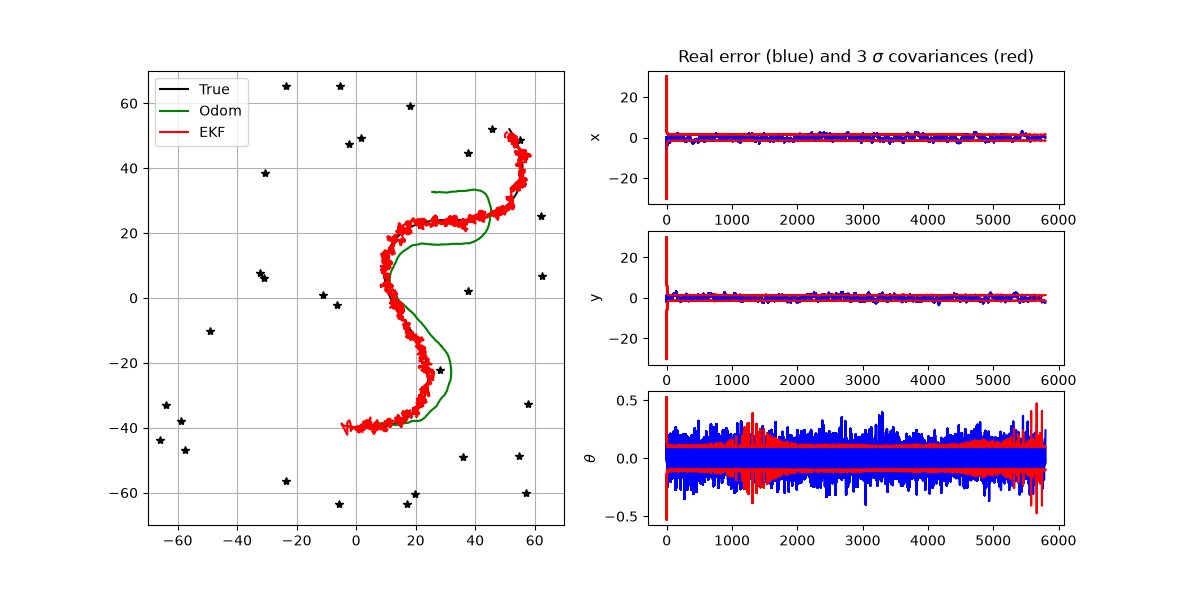
\includegraphics[width=0.95\linewidth]{Q3_Pdiminue_Qaugmente.png}
    \caption{Influence d'une forte surestimation du bruit d'odométrie et
    d'une sous-estimation du bruit des observations.}
    \label{fig:q3_q_augmente}
\end{figure}

On observe que l'estimation reste globalement proche de la trajectoire
réelle. Cependant, les erreurs et les incertitudes sont particulièrement
visibles sur l'orientation $\theta$. Cette situation montre que le filtre
fait fortement confiance aux observations pour corriger la prédiction,
car le bruit de mesure utilisé par le filtre est considéré comme faible.

Nous considérons ensuite le cas demandé dans l'énoncé où le bruit estimé
sur la distance des landmarks est important, tandis que le bruit sur
leur direction reste correct. On utilise :

\[
P_Y^{\mathrm{Est}}
=
\operatorname{diag}
\left(
100^2,
\left(\frac{6\pi}{180}\right)^2
\right).
\]

Le filtre considère alors les mesures de distance comme peu fiables et
leur attribue un poids plus faible. En revanche, les mesures de direction
restent considérées comme fiables et conservent une influence importante
dans la correction.

\begin{figure}[H]
    \centering
    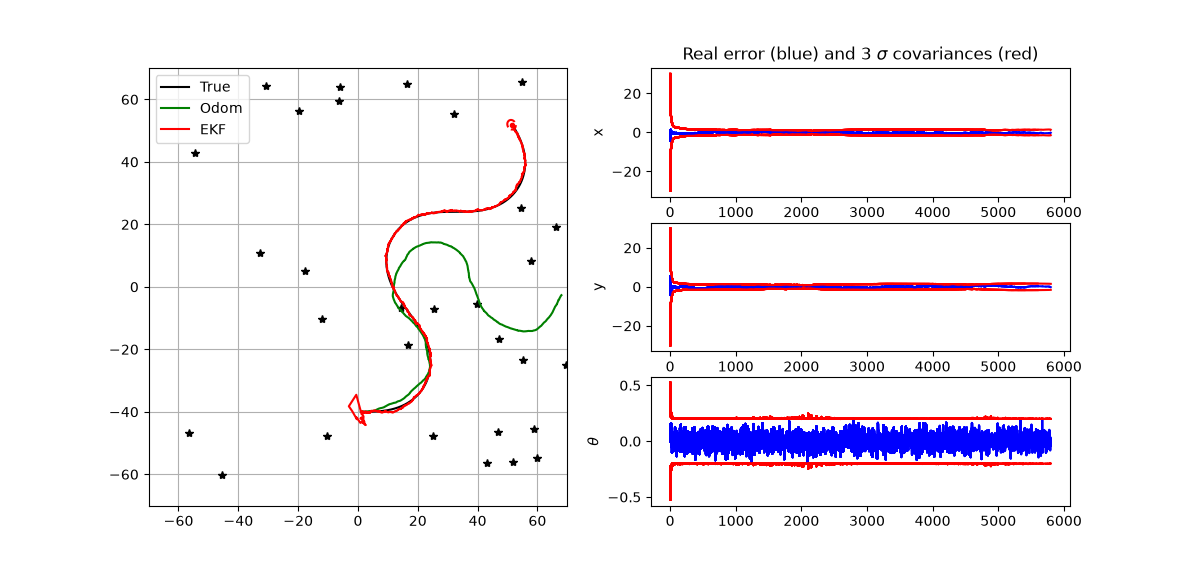
\includegraphics[width=0.95\textwidth]{Q3_distance_large_direction_correct.png}
    \caption{Estimation lorsque le bruit estimé sur la distance des
    landmarks est important tandis que le bruit sur leur direction reste
    correct.}
    \label{fig:q3_distance_large}
\end{figure}

On observe que la trajectoire estimée reste proche de la trajectoire
réelle malgré la forte incertitude sur les distances. Les informations
angulaires permettent en effet de continuer à corriger l'estimation,
notamment l'orientation. La distance n'est pas supprimée de
l'observation, mais son influence dans la correction est fortement
réduite.

Ainsi, une mauvaise estimation des matrices de covariance modifie
directement le compromis entre la prédiction et les observations. Le
filtre accorde plus ou moins de confiance à chaque source d'information
en fonction des valeurs de $Q_{\mathrm{Est}}$ et
$P_Y^{\mathrm{Est}}$.

\section{Q2.4 --- Observabilité partielle}

Dans cette expérience, on étudie le comportement de l'EKF lorsque
seule une partie de l'observation des landmarks est disponible.
On considère successivement le cas où seule la distance est utilisée,
puis celui où seule la direction est utilisée.

\begin{figure}[H]
    \centering
    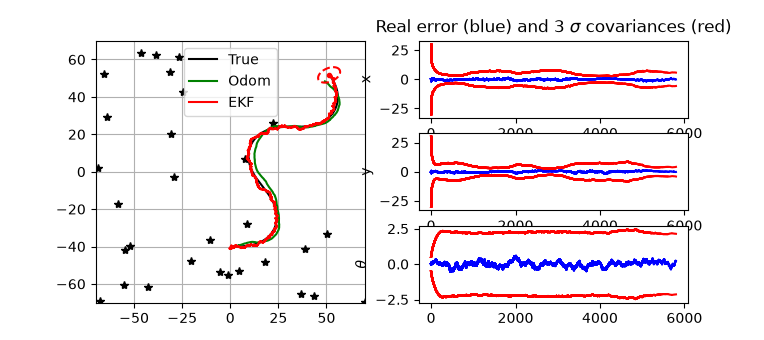
\includegraphics[width=0.95\textwidth]{Q4_distance.png}
    \caption{Estimation avec uniquement la distance aux landmarks.}
    \label{fig:q4_distance}
\end{figure}

Lorsque seule la distance est utilisée, l'observation est donnée par :

\[
z = r =
\sqrt{(x_L-x)^2+(y_L-y)^2}.
\]

La distance fournit une information sur la position du robot par rapport
aux landmarks, mais elle ne dépend pas directement de son orientation
$\theta$. Sur la figure, on observe néanmoins que l'estimation de la
trajectoire reste proche de la trajectoire réelle et que les erreurs sur
$x$ et $y$ restent faibles.

En revanche, l'incertitude sur $\theta$ est plus importante. L'orientation
est donc moins directement observable avec la distance seule et doit être
estimée en partie grâce au modèle dynamique et aux observations
successives.

\begin{figure}[H]
    \centering
    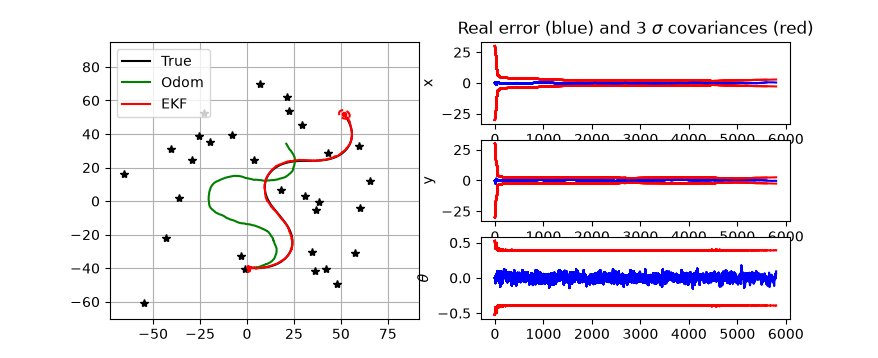
\includegraphics[width=0.95\textwidth]{Q4_direction.png}
    \caption{Estimation avec uniquement la direction des landmarks.}
    \label{fig:q4_direction}
\end{figure}

Dans le second cas, seule la direction du landmark est utilisée :

\[
z = \theta_L-\theta.
\]

Cette observation contient directement une information sur l'orientation
du robot. La figure montre que la trajectoire estimée reste également
proche de la trajectoire réelle et que les erreurs sur $x$ et $y$ restent
faibles.

L'effet est particulièrement visible sur $\theta$ : la bande
d'incertitude $3\sigma$ est nettement plus faible que dans le cas de la
distance seule. L'orientation est donc mieux contrainte lorsque la
direction du landmark est mesurée directement.

Ainsi, la distance et la direction fournissent des informations
complémentaires : la distance contraint principalement la position,
tandis que la direction apporte davantage d'information sur
l'orientation. Dans les deux cas, l'EKF reste capable de suivre la
trajectoire, mais avec une incertitude différente selon la composante
observée.

\section*{Conclusion}

Au fil de ce rapport, le filtre de Kalman s'est révélé un outil efficace pour la localisation,
mais avec des limites bien identifiées. Le filtre linéaire converge rapidement, alors que l'EKF,
privé d'une information suffisante (mesure d'angle seule), peut diverger. Les trous de mesure
font croître l'incertitude -- quadratiquement pour la position en GNSS, cubiquement dans le cas
de l'odométrie -- jusqu'au retour des observations. Enfin, le réglage des covariances $Q$ et $R$
conditionne directement le compromis entre confiance accordée au modèle et confiance accordée aux
mesures : un mauvais choix dégrade sensiblement l'estimation.

\end{document}
